% DSD Lab5 report

\documentclass[10pt]{article}
\usepackage{mathtools, amsmath, amsfonts, amssymb}
\usepackage{hyperref, graphicx, wrapfig, geometry}
\usepackage[makeroom]{cancel}

\usepackage[section]{placeins}
\newgeometry{margin=2cm}

\title{ECSE 323 --- Group 47 Lab 5 Enigma Machine}
\author{Jun Young Shin id. 260499663\\ Timothee Flichy id. 260557686}
\date{\today}

\begin{document}
\maketitle
\section{Introduction}
The enigma machine is a cipher machine which encrypts a string of words or numbers so that a non partisan will not be able to understand the message. This system was extensively used during the world war 1 and 2 by Germany to plan strategic assault to enemy territory. to encrypt the message, the machine used a set of mechanical rotors and electrical circuit. The each rotor can be set by rotating the rotor and ring, and by changing the encryption type. In total, there is 3 independent rotors. In the electrical circuit, there is a circuit called a reflect and sketcher which creates another level of encryption by generation a secondary pattern. This complex encryption system is able to create over 158 million million million combinations with 10 pairs of 26 letters. This makes it almost impossible for a human to decrypt the code. To make it even harder and increase the odd, the combination was changed every 24 hours during world war 2. In the course of Digital System Design, we used VHDL to write electronic version of this mechanical system. This report will explain the procedure of creating this device using the Altera board.

\section{Designing of the Enigma machine}
Before jumping into the VHDL, we first must understand how to implement the mechanical machine to a hardware. In our case the Altera's Cyclone II FPGA model EP2C20F484C7. In figure \ref{fig:enigma_machine_BD} we can see how the hardware will work.
\begin{figure}[!htb]
    \centering
    \includegraphics[width=0.7\textwidth]{./enigma_machine_BD.png}
    \caption{Block diagram of the enigma machine.}
    \label{fig:enigma_machine_BD}
\end{figure}

So here is how the enigma machine will work on the FPGA. The user inputs a letter to be encrypted. When the user click a button called a key\_press, the program receives the letter and sends it to the sketcher. Sketcher meaning plugboard in German, is a simple version of a fixed rotor. It then passes through the first rotor to get the first encryption. The encryption pattern in shown in figure \ref{fig:rotor_encryption}. The encrypted letter will then pass to the second rotor and to the third rotor.
\begin{figure}[!htb]
    \centering
    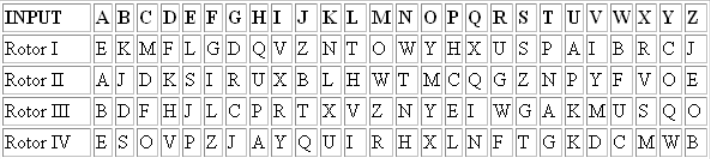
\includegraphics[width=0.7\textwidth]{./rotor_encryption.png}
    \caption{Encryption pattern for the rotor.}
    \label{fig:rotor_encryption}
\end{figure}
It will then pass to the reflector which does another encryption. The reflector will encrypt the letter to a mirrored letter. Meaning, if $'A'$ is mirrored with $'Y'$, if any of the letter is passed to the reflector, the mirrored letter will to output it. The encryption of the reflector can be seen in figure \ref{fig:reflector_encryption}.
\begin{figure}[!htb]
    \centering
    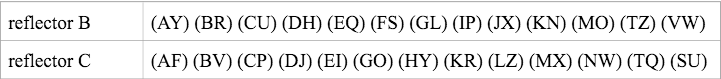
\includegraphics[width=0.7\textwidth]{./reflector_encryption.png}
    \caption{Encryption pattern for the reflector.}
    \label{fig:reflector_encryption}
\end{figure}
The reflected letter will then pass back to the third rotor, to the second rotor, and to the first rotor. It finally come back to the sketcher which output the encrypted letter.\\ 
The user will initialize the enigma machine. There are multiple setting that can be configured.

\section{User Interface}





\end{document}